\subsection{Path planning and Control}

\begin{figure}[h]
\centering
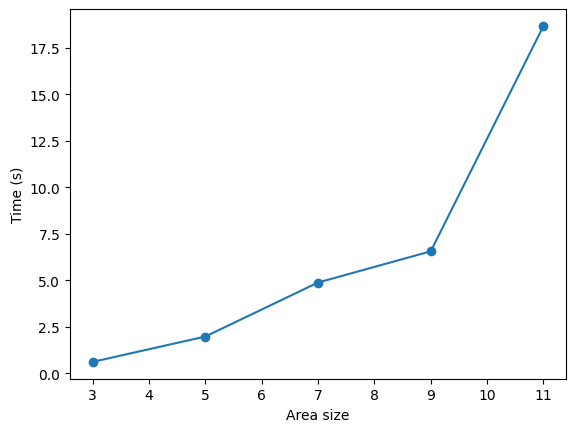
\includegraphics[scale=0.5]{images/time_area.png}
\caption{Area to explore vs time for finding path}
\end{figure}


As shown in Figure 3, the computation time tends to increase exponentially with area, and so we've solved RRTs on smaller areas.
The total time combined for solving RRTs on smaller maps is lesser than finding a path on the entire area.

RRTs produce a collision-free path, but they are neither smooth nor optimal.
A smooth path that adheres to the differential flatness property of a drone (i.e., four times differentiable) will allow us to directly calculate the required rotor torques for controlling the drone.
Using this information, a better controller with feed-forward control can be implemented.
Webb et al. introduced a Kindodynamic $RRT^*$ algorithm that exactly and optimally connects any pair of states for any system with controllable linear dynamics in state spaces of arbitrary dimensions\cite{DBLP:journals/corr/abs-1205-5088}.
With this improvement, the drone can fly faster and cover more distance as well.
In terms of improvements, the differential flatness property of a drone can be exploited to control motion upto the fourth derivative and generate smoother paths and simplifying trajectory generation.

 
\subsection{Global planner}

The global planner provides a series of goals for every drone in the global frame, scouting the entire region. This is done by converting the grid into cells and providing separate paths for each drone to visit. This is indeed practical and efficient as it provides continuous cell path by covering immediate neighbouring cells.

In practice, the global planner could use a satellite image of a forest and plan drones to cover it. 


\subsection{Local maps}

To reduce overall computation time, RRT computes multiple obstacle free paths
using a series of local maps to reach the global goal. This is done by slicing sections of the global occupancy map just enough to include the next goal given by the global planner to avoid use of a global occupancy map. The area vs time figure clearly shows that local maps of small areas combined would take shorter time to compute compared to the exponential increase of using a single global map.

\subsection{Obstacle detections}
With that said, all obstacles are revealed within a local map for the drone to compute a obstacle free path. The local map's dimensions can differ depending on the global map and grid size, which means detecting all obstacles within a local map is unlikely in the real world where sensors have a limited range of detection. \\
 A potential improvement here to imitate a real world scenario is using a dynamic local map and revealing obstacles only within a certain radius of the drone.

